\documentclass[a4paper, 11pt]{article}
\usepackage{comment}
\usepackage{lipsum} 
\usepackage{fullpage} %cambiar margen
\usepackage[a4paper, total={7in, 10in}]{geometry}

\usepackage{amssymb,amsthm} 
\usepackage{amsmath}
\newtheorem{theorem}{Theorem}
\newtheorem{corollary}{Corollary}
\usepackage{graphicx}
\usepackage{tikz}
\usetikzlibrary{arrows}
\usepackage{verbatim}
%\usepackage[numbered]{mcode}
\usepackage{float}
\usepackage{tikz}
\usetikzlibrary{shapes,arrows}
\usetikzlibrary{arrows,calc,positioning}
\usepackage{mathpazo} %tipo de letra 
\usepackage[utf8]{inputenc} %codificación
\usepackage[T1]{fontenc} %digitación de tildes y ñ
\usepackage[spanish]{babel} %paquete de soporte español

\tikzset{
	block/.style = {draw, rectangle,
		minimum height=1cm,
		minimum width=1.5cm},
	input/.style = {coordinate,node distance=1cm},
	output/.style = {coordinate,node distance=4cm},
	arrow/.style={draw, -latex,node distance=2cm},
	pinstyle/.style = {pin edge={latex-, black,node distance=2cm}},
	sum/.style = {draw, circle, node distance=1cm},
}
\usepackage{xcolor}
\usepackage{mdframed}
\usepackage[shortlabels]{enumitem}
\usepackage{indentfirst}
\usepackage{hyperref}

\usepackage{listings}
\lstset{literate=
  {á}{{\'a}}1
  {é}{{\'e}}1
  {í}{{\'i}}1
  {ó}{{\'o}}1
  {ú}{{\'u}}1
  {Á}{{\'A}}1
  {É}{{\'E}}1
  {Í}{{\'I}}1
  {Ó}{{\'O}}1
  {Ú}{{\'U}}1
  {ñ}{{\~n}}1
  {ü}{{\"u}}1
  {Ü}{{\"U}}1
}

\lstdefinestyle{customc}{
  belowcaptionskip=1\baselineskip,
  breaklines=true,
  frame=L,
  xleftmargin=\parindent,
  language=Python,
  showstringspaces=false,
  basicstyle=\footnotesize\ttfamily,
  keywordstyle=\bfseries\color{green!40!black},
  commentstyle=\itshape\color{purple!40!black},
  identifierstyle=\color{blue},
  stringstyle=\color{orange},
}

\lstdefinestyle{customasm}{
  belowcaptionskip=1\baselineskip,
  frame=L,
  xleftmargin=\parindent,
  language=[x86masm]Assembler,
  basicstyle=\footnotesize\ttfamily,
  commentstyle=\itshape\color{purple!40!black},
}

\lstset{escapechar=@,style=customc}



\renewcommand{\thesubsection}{\thesection.\alph{subsection}}

\newenvironment{problem}[2][Ejercicio]
{ \begin{mdframed}[backgroundcolor= red!50] \textbf{#1 #2} \\}
	{  \end{mdframed}}

% Define solution environment
\newenvironment{solution}
{\textcolor{blue}{\textbf{\textit{Solución:\\\noindent}}}}


\renewcommand{\qed}{\quad\qedsymbol}

% \\	
\begin{document}
	\noindent
	%%%%%%%%%%%%%%%%%%%%%%%%%%%%%%%%%%%%
	
	\begin{minipage}[b][1.2cm][t]{0.8\textwidth}
		\large\textbf{César Isaí García Cornejo} \hfill \textbf{Tarea 6}  \\
		cesar.cornejo@cimat.mx \hfill \\
		\normalsize Computo Científico \hfill Semestre 3\\
	\end{minipage}
	
	\hspace{14.4cm}
	\begin{minipage}[b][0.03cm][t]{0.12\linewidth}
		
		\vspace{-2.2cm}
		%%%La Ruta dependerá de donde este alojado el main y la imagen
		
\includegraphics[scale=0.3]{Figures/EscudoCimat.png}
	\end{minipage}
	
	\noindent\rule{7in}{2.8pt}
	
	%%%%%%%%%%%%%%%%%%%%%
	%%%%%%%%%%%%%%%%%%%%%%%%%%%%%%%%%%%%%%%%%%%%%%%%%%%%%%%%%%%%%%%%%%%%%%%%%%%%%%%%%%%%%%%%%%%%%%%%%%%%%%%%%%%%%%%%%%%
	% Problem 1
	%%%%%%%%%%%%%%%%%%%%%%%%%%%%%%%%%%%%%%%%%%%%%%%%%%%%%%%%%%%%%%%%%%%%%%%%%%%%%%%%%%%%%%%%%%%%%%%%%%%%%%%%%%%%%%%%%%%%%%%%%%%%%%%%%%%%%%%%
	\setlength{\parskip}{\medskipamount}
	\setlength{\parindent}{0pt}
%/////////// Ejercicio 1 /////////////////

    
\begin{problem}{1} 
    Simular $n=5$ y $n=40$ v.a. Bernoulli $Be(1/3)$; sea $r$ el número de éxitos en cada caso.
\end{problem}

\begin{solution} 
    Dado que esta simulación influye en el resto de los ejercicios. Consideremos dos semillas. Es decir, haremos dos veces este ejercicio con fines didácticos en el resto de la tarea.

    Considerando la primer semilla (\textbf{rnd = 2} del código).
    
    Para poder hacer una simulación de una Bernoulli$(1/3)$ consideramos una variable aleatoria $y$ uniforme(0,1). Si $y$ es menor que $1/3$ entonces tendremos un éxito, de lo contrario lo contamos como un fracaso. Para hacer la simulación de $n$ variables aleatoria Bernoulli$(1/3)$ ciclamos $n$ veces y guardamos. 

    Para $n= 5$ tenemos el siguiente vector de resultados
    \begin{align*}
      [0. 1. 0. 0. 0.]
    \end{align*}
    Luego, la cantidad de éxitos es $r = 1$.

    Para $n = 40$ tenemos el siguiente vector de resultados
    \begin{align*}
      [0. 1. 0. 0. 0. 1. 1. 0. 1. 1. 0. 0. 1. 0. 1. 0. 0. 0. 0. 1. 0. 1. 0. 1. 1. 0. 1. 1. 1. 0. 0. 1. 0. 0. 0. 0. 0. 0. 1. 0.]
    \end{align*}
    Luego, la cantidad de éxitos es $r= 16$.

    Para la segunda semilla (\textbf{rnd = 4}), obtenemos que para $n = 5$ y $n = 40$ la cantidad de $r = 0$ y $r = 12$ éxitos, respectivamente.
\end{solution}

\begin{problem}{2} 
    Implementar el algoritmo Metropolis-Hastings para simular de la posterior
    \begin{align*}
        f(p|\bar{x }) \propto p^r (1-p )^{n-r } cos(\pi p ) I_{[0,\frac{1}{2}]}(p),
    \end{align*}
    con los dos casos de $n$ y $r$ de arriba. Para ello poner la propuesta $(p'|p ) = p' \sim Bete(r+1,n-r+1)$ y la distribución inicial de la cadena $\mu \sim U(0,\frac{1}{2})$
\end{problem}

\begin{solution} 
  
Para la implementación del método de Metropolis-Hastings, se creo una función que recibe el $n,r$ de la distribución objetivo. Además recibe la cantidad de iteraciones que se desea aplicar así como la distribución objetivo dada por el enunciado y la distribución propuesta que es la distribución beta también dada por el enunciado.

Como se puede ver en el código correspondiente, se toma un punto inicial $x_0$ con distribución uniforme(0,1/2). Luego, según la distribución propuesta (condicional) se propone un nuevo valor. La distribución propuesta predeterminada es la Beta$(n+1,n-r+1)$. Una vez que se simula de la distribución propuesta, se hace un ensayo Bernoulli de parámetro $\rho$
\begin{align*}
  \rho = \min\left \{ 1, \frac{f(y)q(x|y)}{f(x)q(y|x)} \right \}
\end{align*}
como la distribución propuesta para este ejercicio es independiente del valor actual en la cadena, entonces $q(x|y) = q(x)$ para todo $x \in $ Supp(f). Iteramos tantas veces como se desea para la cadena de Metropolis-Hastings y regresamos los valores obtenidos en cada paso de dicha cadena.

Para la primer semilla \textbf{rnd = 2}. Tenemos que simular de la distribución objetivo con los parámetros n y r ya especificados

Iteramos 20,000 veces y graficamos el histograma junto a su función de densidad objetivo. Mostrando los resultados en la siguiente Figura.
\begin{figure}[H] 
    \centering 
    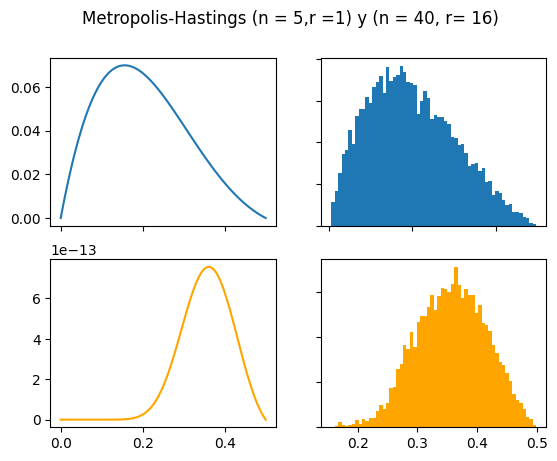
\includegraphics[width = 14 cm ]{Figures/Metropolis.png} 
    \caption{De la primer fila de izquierda a derecha (azul). La función de densidad objetivo con n=5 y r=1 y el histograma generado por 20000 pasos en la cadena de Metropolis-Hastings. De la segunda fila (naranja), la densidad objetivo con n = 40 y r = 16 además de el histograma generado con la misma cantidad de iteraciones por M-H.}
    \label{Fig. 2.1}
\end{figure} 

Para la segunda semilla \textbf{rnd = 4}. Tenemos una distribución objetivo con $n = 5$ y $r = 0$. También la función objetivo $n = 40$ $r = 12$. Nuevamente, tras 20,000 iteraciones tenemos la siguiente Figura
\begin{figure}[H] 
    \centering 
    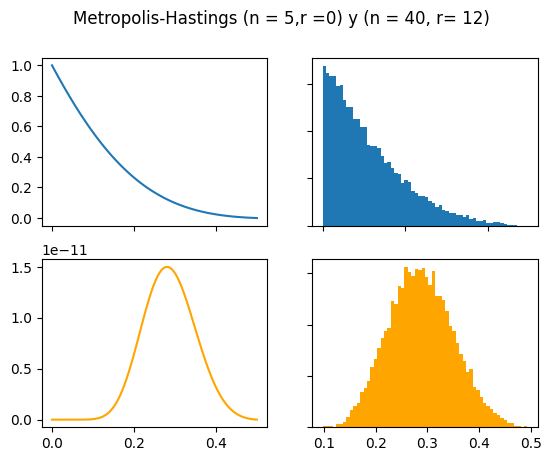
\includegraphics[width = 14 cm ]{Figures/Metropolis2.png} 
    \caption{De la primer fila de izquierda a derecha (azul). La función de densidad objetivo con n=5 y r=0 y el histograma generado por 20000 pasos en la cadena de Metropolis-Hastings. De la segunda fila (naranja), la densidad objetivo con n = 40 y r = 12 además de el histograma generado con la misma cantidad de iteraciones por M-H.}
    \label{Fig. 2.2}
\end{figure} 

Notemos que tenemos un excelente ajuste para la distribución objetivo asociada a $n =5 $ (azul). Sin embargo, no podemos decir lo mismo para la distribución asociada a $n = 40$ (naranja). La falta de ajuste a la distribución naranja se debe a dos causas. La primera, es sobre las escalas que maneja la densidad, ya que tenemos que elevar cantidades a la $n = 40$ y a la $n-r = 24$ lo que conlleva a error computacional. La segunda, se debe a la cantidad de veces que la cadena de Markov se queda \textit{atorada} en el mismo estado. Si la cantidad de rechazos es alta, entonces la muestra tenderá a tener más peso en dicha parte.

Analizando a la cadena de Markov de Metropolis-Hastings, graficamos los saltos de la cadena como una serie de tiempo y vemos su comportamiento. Para \textbf{rnd = 2}
\begin{figure}[H] 
    \centering 
    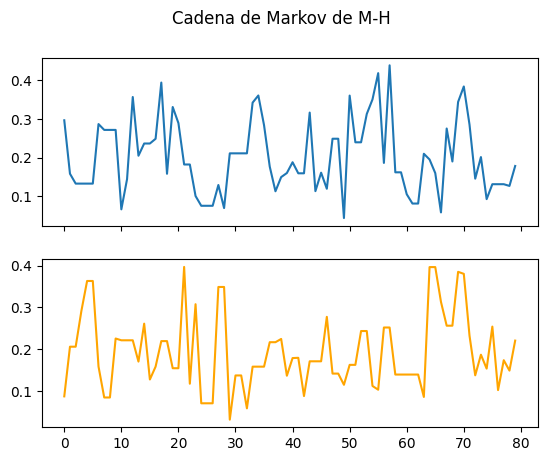
\includegraphics[width = 12 cm  ]{Figures/Cadena.png}   
    \caption{Cadena de saltos en el tiempo para cada uno de las distribuciones objetivo para la primer semilla.}
    \label{Fig. 2.3}
\end{figure} 
Mientras que para \textbf{rnd = 4}
\begin{figure}[H] 
    \centering 
    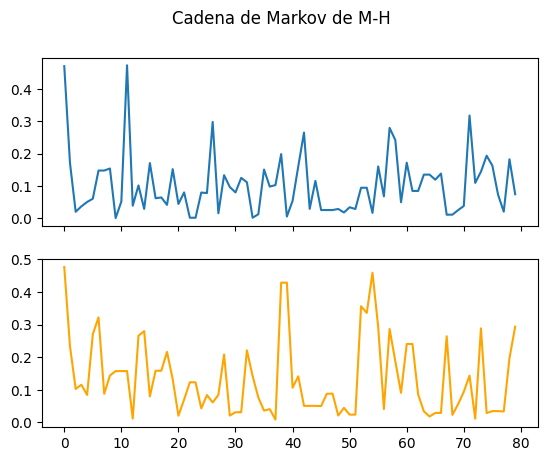
\includegraphics[width = 12 cm  ]{Figures/Cadena2.png} 
    \caption{Cadena de saltos en el tiempo para cada uno de las distribuciones objetivo para la segunda semilla.}
    \label{Fig. 2.4}
\end{figure} 
Observemos que para la cadena (naranja) en ambas semillas tiene más rechazos, sobre todo la cantidad de rechazos se muestra en las colas, lo que justifica la desviación respecto a la distribución objetivo.

\end{solution}

\begin{problem}{3} 
    Argumentar porque la cadena es $f$-irreducible y porque es ergódica. Implementar el algoritmo con los datos descritos y discutir los resultados.
\end{problem}

\begin{solution} 
  
Consideremos un conjunto $A$ de tal forma que $f(A) >0 $ donde $f$ es la distribución objetivo, es decir $A \in $ Supp(f). Notemos que $A \subset (0,1/2)$. Debido a que la distribución propuesta es independiente del actual estado de la cadena, es decir $q(y|x) = q(y)$. La cadena saltará en el siguiente paso con proba positiva si $y \in A$ de otra forma se quedará en el mismo estado hasta que el siguiente tiempo se proponga saltar a una nueva simulación y. Entonces podemos ver que, como eventualmente la distribución beta tendrá una realización en (0,1/2) y el ensayo Bernoulli será éxito, se sigue que existe $n$ tal que el kernel $K(x,y)$ (o probabilidad/densidad de transición del estado $x$ a $y$) es positivo para un tiempo $n$, es decir
\begin{align*}
  K^n(x,y) > 0  \:\:\:\: \text{para algún} \:\:n
\end{align*}
Que es la definición de una cadena f-irreducible.

Ahora, notemos que $K(y,y) >0$ para todo $y \in A$ ya que $\rho > 0 $. Dicho de otra forma, existe proba positiva de quedarse en el mismo estado, para aquellos estados que pertenecen al soporte de $f$. Entonces, la cadena es fuertemente aperiodica. Y junto a la f-irreducibilidad, se sigue que la cadena es ergódica. 

\end{solution}

\begin{problem}{4} 
    Implementar el algoritmo Metropolis-Hastings con la posterior de arriba tomando una propuesta diferente.
\end{problem}

\begin{solution} 
    Se ajusto el código para poder hacer un cambio en la distribución propuesta. Esta vez tomaremos como distribución propuesta a la distribución uniforme en (0,1/2). Dicha distribución es simétrica por lo que 
    \begin{align*}
      \rho = \min\left \{ 1, \frac{f(y)}{f(x)} \right \}
    \end{align*}

    Dentro del código solo basta poner en la función MetropolisHastings(n,r, propuesta = 'Uniforme') explícitamente.
    
    Para ambos casos de las semillas, esbozamos la gráfica de la distribución y su muestreo por M-H para 20000 iteraciones de la cadena.
    \begin{figure}[H] 
        \centering 
        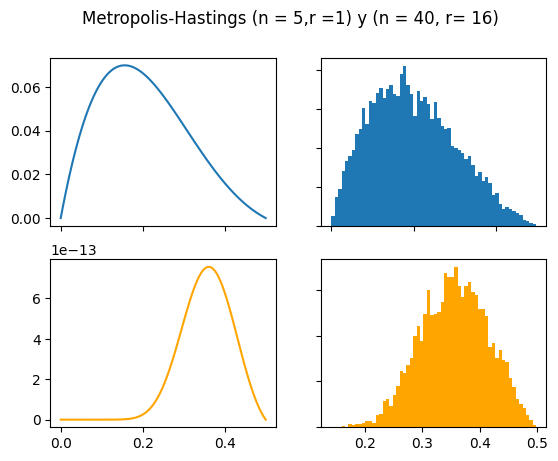
\includegraphics[width = 14 cm ]{Figures/MetropolisProuesta.png} 
        \caption{De la primer fila de izquierda a derecha (azul). La función de densidad objetivo con n=5 y r=0 y el histograma generado por 20000 pasos en la cadena de Metropolis-Hastings con distribución propuesta uniforme. De la segunda fila (naranja), la densidad objetivo con n = 40 y r = 12 además de el histograma generado con la misma cantidad de iteraciones por M-H.}
        \label{Fig. 4.1}
    \end{figure} 

    Para la semilla \textbf{rnd = 4} tenemos la siguiente simulación 
    \begin{figure}[H] 
        \centering 
        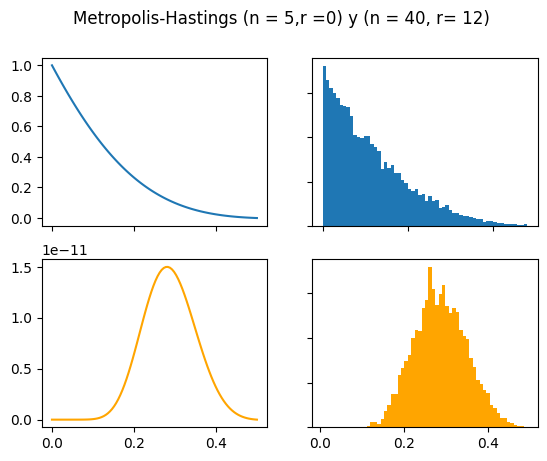
\includegraphics[width = 14 cm ]{Figures/Metropolis2Propuesta.png} 
        \caption{De la primer fila de izquierda a derecha (azul). La función de densidad objetivo con n=5 y r=0 y el histograma generado por 20000 pasos en la cadena de Metropolis-Hastings con distribución propuesta uniforme. De la segunda fila (naranja), la densidad objetivo con n = 40 y r = 12 además de el histograma generado con la misma cantidad de iteraciones por M-H.}
        \label{Fig. 4.2}
    \end{figure} 
    Vemos una ligera reducción del ajuste del histograma a la función de densidad. Pese a esto, aún tenemos una simulación plausible para la función de densidad objetivo. Por lo que hemos visto, la distribución propuesta beta es superior a la uniforme en el sentido de que la convergencia a la distribución objetivo es más rápida.

    Para la serie de tiempo de la cadena de saltos de Metropolis-Hastings para la primer semilla
    \begin{figure}[H] 
        \centering 
        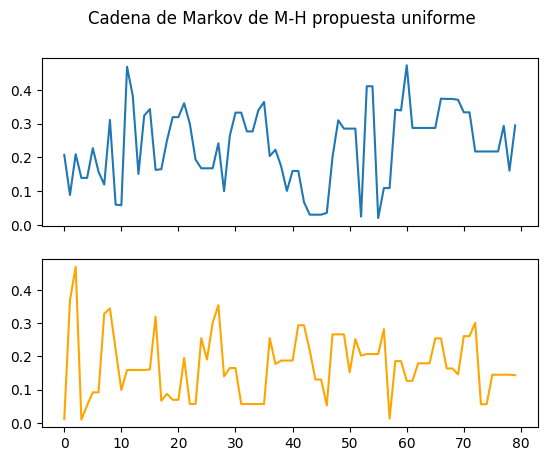
\includegraphics[width = 12 cm ]{Figures/CadenaPropuesta.png} 
        \caption{Cadena de saltos en el tiempo para cada uno de las distribuciones objetivo para la primer semilla.}
        \label{Fig. 4.3}
    \end{figure} 
    y para la segunda semilla
    \begin{figure}[H] 
        \centering 
        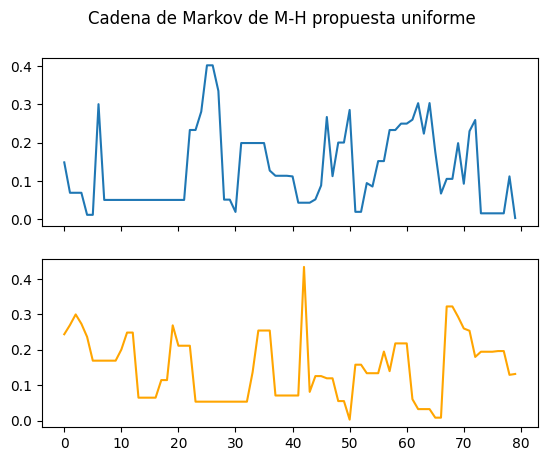
\includegraphics[width = 12 cm ]{Figures/Cadena2Propuesta.png} 
        \caption{Cadena de saltos en el tiempo para cada uno de las distribuciones objetivo para la segunda semilla.}
        \label{Fig. 4.4}
    \end{figure} 
    
    De estas series, es claro que la cadena se atora bastante más de lo que lo hacía con respecto a la distribución propuesta de la beta. Estos valores donde la cadena es constante se muestra en las colas pesadas del histograma lo que explica su diferencia con la distribución objetivo.

\end{solution}

\begin{thebibliography}{9}

    \bibitem{Casella}
    Robert, C. P., Casella, G., and Casella, G. (1999). Monte Carlo statistical methods (Vol. 2). New York: Springer.

    \bibitem{Wasserman}
    Wasserman, L. (2004). All of statistics: a concise course in statistical inference (p. 413). New York: Springer.
    
\end{thebibliography}
      




    \end{document}